\documentclass[parskip=full,11pt]{scrartcl}

\usepackage[sfdefault,light]{roboto}
\usepackage{inconsolata}
\usepackage[ngerman]{babel}

\usepackage[utf8]{inputenc}
\usepackage[T1]{fontenc}

\usepackage{microtype}

\usepackage{csquotes}
\MakeOuterQuote{"}

\usepackage{graphicx}
\usepackage{float}
\usepackage{bm}
\usepackage{amssymb}
\usepackage[hidelinks]{hyperref}
\usepackage[section]{placeins}


\usepackage[T1]{fontenc}
\usepackage[scaled=0.85]{beramono}

\begin{document}
\begin{titlepage}
	\centering
	\vspace*{5cm}
	
\includegraphics[width = 0.7\linewidth]{img/logo.png}\par
	{\huge\bfseries Ein Simulator für wiederholte Spiele\par}
	%\vspace{1cm}
	{\Large Implementierungsbericht\par}
	\vspace{2cm}
	{\Large\itshape Sebastian Feurer, Peter Koepernik, Luc Mercatoris,\\Christian Schorr, Pierre Toussing\par}
	\vfill
	{\large \today\par}
\end{titlepage}

\tableofcontents
\pagebreak

\section{Einleitung}
Nach der Spezifikation des Programms in der ersten und dem Entwurf einer Programmarchitekur in der zweiten wurde das Programm in dieser Phase nun implementiert. Der Ablauf und die Ergebnisse der Implementierungsphase sollen hier kurz vorgestellt werden.

Innerhalb der letzten vier Wochen wurden durch insgesamt über X Commits im Versionierungssystem git X Klassen und Schnittstellen in X Paketen implementiert, welche  insgesamt X Java-Quellcode-Zeilen umfassen. Des Weiteren wurden zahlreiche Komponententests erstellt.

Im Laufe der Implemetierung sind viele verschiedene Bibliotheken und Programme zum Einsatz gekommen, die hier kurz vorgestellt werden sollen.

\subsection{Gradle}
\begin{enumerate}
\item[] \textbf{Ziel:} Automatisierung des Build-Prozesses
\item[] \textbf{Beschreibung:} Gradle ist ein Build-Management-Automatisierungs-Tool zum automatischen Erstellen ausführbarer Anwendungsprogramme aus Java-Quellcode.
\item[] \textbf{Erläuterung:} Zur Automatisierung des Build-Prozesses und zum vereinfachten Dependency-Management bei Verwendung externer Bibliotheken bietet sich der Einsatz eines Build-Tools an. Wir entschieden uns dabei für Gradle.
\end{enumerate}
\subsection{Eclipse und IntelliJ}
\begin{enumerate}
\item[] \textbf{Ziel:} Bereitstellung eines Editors.
\item[] \textbf{Beschreibung:} Eclipse sowie IntelliJ sind Open-Source-Code-Editoren.
\item[] \textbf{Erläuterung:} Ein Editor ist für das Erstellen eines Programms unerlässlich, da er die Organisation des Projekts, das Erstellen von Klassen und Schnittstellen, das Finden von Fehlern und automatische Ausführen von Tests sowie das Kompilieren erleichtert. Je nach bisherigen Erfahrungen entschieden sich die Entwickler dabei für Eclipse oder IntelliJ.
\end{enumerate}
\subsection{JUnit}
\begin{enumerate}
\item[] \textbf{Ziel:} Testen von Komponenten
\item[] \textbf{Beschreibung:} JUnit ist ein Test-Framework für Java.
\item[] \textbf{Erläuterung:} Für das Testen einzelner Klassen und Interfaces, besonders zur Vermeidung von Regressionen, ist ein Framework nützlich, dass das automatische Ausführen von Komponententests erlaubt.
\end{enumerate}
\subsection{JavaFX}
\begin{enumerate}
\item[] \textbf{Ziel:} Erstellen einer ansprechenden Benutzeroberfläche.
\item[] \textbf{Beschreibung:} JavaFX ist ein Framework zur Erstellung von Benutzeroberflächen für Java-Applikationen.
\item[] \textbf{Erläuterung:} Als GUI-Frameworks kamen zu Beginn Swing und JavaFX in Frage. Da einer der Entwickler bereits in früheren Projekten Erfahrung mit JavaFX gesammelt hat, haben wir uns für dieses Framework entschieden.
\end{enumerate}
\subsection{ControlsFX}
\begin{enumerate}
\item[] \textbf{Ziel:} Bereitstellung weiterer GUI-Elemente
\item[] \textbf{Beschreibung:} ControlsFX ist eine GUI-Bibliothek, die JavaFX ergänzt.
\item[] \textbf{Erläuterung:} Einige der verwendeten GUI-Elemente sind in JavaFX nicht enthalten und werden von ControlsFX bereitgestellt.
\end{enumerate}
\subsection{JGraphT}
\begin{enumerate}
\item[] \textbf{Ziel:} Bereitstellung eines effizienten Matching-Algorithmus für Graphen
\item[] \textbf{Beschreibung:} JGraphT ist eine Open-Source-Graphbibliothek für Java.
\item[] \textbf{Erläuterung:} In einem der verwendeten Paarbildungsalgorithmen (der \enquote{Paarbildung nach Wunsch}) muss ein Matching auf einem Graphen mit gewichteten Kanten berechnet werden. Da das Entwerfen und Implementieren von Graphenalgorithmen nicht Teil dieses Projekts ist, haben wir dazu auf diese Bibliothek zurückgegriffen.
\end{enumerate}
\subsection{Gson}
\begin{enumerate}
\item[] \textbf{Ziel:} (De-)Serialisierung von Java-Objekten
\item[] \textbf{Beschreibung:} Gson ist eine Open-Source-Java-Bibliothek zum Serialisieren und Deserialisieren von Java-Objekten.
\item[] \textbf{Erläuterung:} Beim Speichern von Simulationsergebnissen wollten wir nicht auf die Java-eigene Serialisierungs-Bibliothek zurückgreifen, da das erzwungen hätte, viele der Klassen im Model serialisierbar zu machen. Das wäre entwurfstechnisch nicht schön, weshalb wir uns entschieden haben, hier auf eine andere Bibliothek zurückzugreifen.
\end{enumerate}
\subsection{Apache Commons Math}
\begin{enumerate}
\item[] \textbf{Ziel:} 
\item[] \textbf{Beschreibung:} Apache Commons Math ist eine Open-Source-Java-Bibliothek, die grundlegende mathematische und statistische Werkzeuge zur Verfügung stellt.
\item[] \textbf{Erläuterung:} Bei der Kapitalinitialisierung von Agenten können diskrete Wahrscheinlichkeitsverteilungen wie die Binomial- oder Poissonverteilung verwendet werden. Für die Generierung von entsprechend verteilten Pseudo-Zufallszahlen haben wir auf diese Bibliothek zurückgegriffen.
\end{enumerate}

\newpage
\section{Änderungen am Entwurf}

\subsection{Hinzufügen des Pakets \texttt{edu.kit.loop.view.historylistview}}
Im ursprünglichen Entwurf gab es zunächst kein View-Paket, was daran liegt, dass das Verhalten der GUI in fxml-Dateien beschrieben ist und die View-Klassen daraus zur Laufzeit erzeugt werden. Es ist daher zunächst nicht notwendig, eigene Klassen für die View zu schreiben.

Wie bereits im Pflichtenheft beschrieben, befindet sich im Hauptfenster eine Liste mit Einträgen für alle gestarteten und geladenen Simulationen, die deren Ausführungsstatus anzeigen. Klickt man auf den Eintrag einer abgeschlossenen Simulation, werden rechts der Liste deren Ergebnisse angezeigt. Zur Umsetzung haben wir das in JavaFX vorhandene Konzept der \texttt{ListView} verwendet. Eine \texttt{ListView} zeigt eine Liste von Elementen (Instanzen des Typs \texttt{ListCell}) an, mit denen der Nutzer durch Auswahl einzelner Einträge interagieren kann. Um die Einträge unseren sehr speziellen Anforderungen anzupassen, war es notwendig, eigene Unterklassen der \texttt{ListCell}-Klasse zu schreiben. Diese befinden sich im Paket \texttt{edu.kit.loop.view.historylistview}.

\subsection{Anpassung der Ausgabe}\label{outputmod}
Die Ausgabe der Strategieverteilung der Agenten sollte im ursprünglichen Entwurf durch ein Kuchendiagramm erfolgen, dass für jede Strategie angibt, wie häufig diese von Agenten im finalen Zustand der Simulation verwendet wird. Statt des Kuchendiagramms gibt es nun ein Diagramm, dass die Entwicklung der Strategieverteilung über den Lauf der Simulation anzeigt. Genauer gesagt bilden die Adaptionsschritte von \(1\) bis zum letzten durchgeführten Adaptionsschritt die x-Achse und es gibt für jede Strategie eine Linie im Diagramm, die für jeden Adaptionsschritt als Wert die relative Verwendungshäufigkeit dieser Strategies in diesem Adaptionsschritt annimmt (siehe Abb. \ref{fig:newoutput}). Die Informationen aus dem ursprünglich geplanten Kuchendiagramm sind in diesem enthalten, die Strategieverteilung nach dem letzten Adaptionsschritt kann im Liniendiagramm ganz rechts abgelesen werden.

\begin{figure}[h]
	\centering
	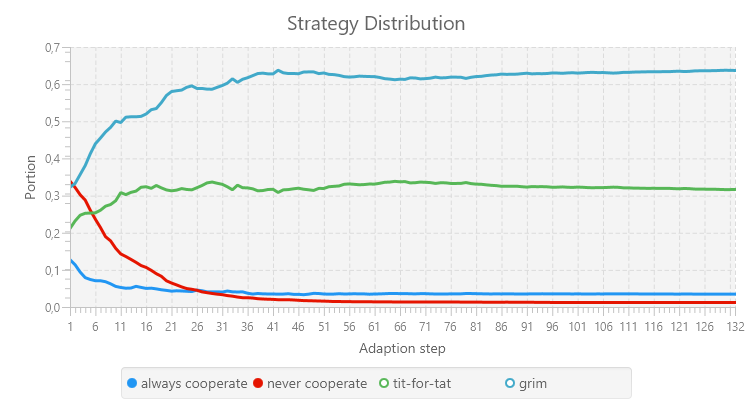
\includegraphics[width=\linewidth]{img/newoutput.png}
	\caption{Bild des neuen Diagramms im Ausgabefenster.}
	\label{fig:newoutput}
\end{figure}

\newpage
\section{Implementierte Funktionalitäten}
Die folgende Tabelle liefert einen Überblick über die im Pflichtenheft beschriebenen Funktionalitäten und deren Umsetzung.

\begin{table}[h]
\centering
\begin{tabular}{l | l | l | l}
\textbf{Nummer} & \textbf{Beschreibung} & \textbf{implementiert?} & \textbf{Bemerkung} \\
\hline
\textbf{M1} & Starten einer Simulation  & \checkmark \\
\textbf{M2} & Ausgabe der Simulationsergebnisse & \checkmark & 1)\\
\textbf{M3} & Abbrechen einer Simulation & \checkmark \\
\textbf{M4} & Festlegung von Simulationsparametern & \checkmark \\
\textbf{K1} & Multikonfiguration &  \checkmark \\
\textbf{K2} & Erstellen eigener Strategien & \checkmark \\
\textbf{K3} & Erstellen eigener Stufenspiele & \checkmark\\
\textbf{K4} & Speichern und Laden von Konfigurationen & \checkmark & 2)\\
\textbf{K5} & Speichern und Laden von Simulationsergebnissen & \checkmark & 2) \\
\textbf{K6} & Starten mehrerer Simulationen & \checkmark \\
\textbf{K7} & Anpassen der Gleichgewichtsbedingung & \checkmark \\
\textbf{K8} & Erweiterte Gruppenfunktionalität & \checkmark & 3) \\
\hline
\textbf{Gesamt} &\textbf{12} & \textbf{12}
\end{tabular}
\caption{Übersicht der implementierten Muss- und Kann-Kriterien}
\end{table}
Wie in der Tabelle zu sehen, konnten alle Kriterien erfolgreich umgesetzt werden, dazu jedoch noch folgende Anmerkungen:
\begin{enumerate}
\item[] 1) Die Form der Ausgabe der Strategieverteilung der Agenten wurde angepasst (siehe Abschnitt \ref{outputmod}).
\item[] 2) Neben Konfigurationen und Simulationsergebnissen können auch Gruppen, Populationen, Strategien und Stufenspiele als Dateien exportiert und importiert werden.
\item[] 3) Die Struktur von Gruppen und Segmenten hat sich in der Entwurfsphase durch die Einführung von Populationen geändert (siehe Entwurfsdokument).
\end{enumerate}

Neben den in der Tabelle erwähnten Funktionen konnten wir auch erfolgreich die Funktionalitäten implementieren, die wir in der Entwurfsphase noch zur Spezifikation hinzugefügt haben, also das Konzept von Populationen, erweiterte Möglichkeiten zur Erstellung von Strategien und das Plugin-System.

\section{Schwierigkeiten bei der Implementierung}

\subsection{Erstellung des Multisliders}

\subsection{Das Plugin-System}
wegen gradle

\section{Implementierungsplan}
Zu Beginn der Implementierungsphase wurde vereinbart, die Aufteilung anhand der Paketstruktur vorzunehmen. Weiterhin erachteten es die Entwickler als sinnvoll, zunächst das Model zu implementieren und zu testen, und erst danach mit Controller und View zu beginnen. Grund ist eine Vereinfachung der Fehlersuche bei der Implementierung des Controllers. Ist dann nämlich das Model bereits fertig implementiert und getestet und es entsteht ein Fehler in einem Ablauf, in dem sowohl Controller als auch Model beteiligt sind, so liegt der Fehler höchstwahrscheinlich im Controller. Diese Vorgehensweise hat sich bewährt.

Bei der Implementierung des Models sind wir so vorgegangen, dass wir das aus fünf Entwicklern bestehende Team aufgeteilt haben in drei, die mit der Implementierung der Model-Pakete beginnen und zwei, die parallel Komponententests dazu schreiben. Die Implementierung des Models verlief reibungslos und war bereits nach etwa eineinhalb Woche abgeschlossen.

Während die zwei Tester noch weiter an Komponententests für das Model arbeiteten, begonnen die anderen drei Entwickler mit der Implementierung des Controllers und dem Anfertigen der fxml-Dateien für die View. Da die meisten Entwickler keine Erfahrung im Umgang mit JavaFX hatten, stellte sich diese Phase als etwas zeitaufwendiger heraus, verlief aber auch ohne Probleme.

\end{document}